\documentclass{beamer}
\usepackage{../tut-slides}
\usepackage{../mathoperatorsAuD}

\usepackage{amsmath,amssymb}
\usepackage{stmaryrd}
\usepackage{enumerate}
\usepackage{csquotes}
%\usepackage[inline]{enumitem} 		%customize label
%\newcommand{\labelitemi}{\raisebox{1pt}{\scalebox{.9}{$\blacktriangleright$}}}
%\newcommand{\labelitemii}{$\vartriangleright$}
%\newcommand{\labelitemiii}{--}
\setbeamertemplate{itemize item}{\raisebox{1pt}{\scalebox{.9}{$\blacktriangleright$}}}
\setbeamertemplate{itemize subitem}{$\vartriangleright$}

\usepackage{booktabs}
\usepackage{tabularx}
\usepackage{tabu}
\newcommand*\head{\rowfont{\bfseries}}
\newcommand*{\tw}{\rowfont{\ttfamily}}
\renewcommand{\tabularxcolumn}[1]{>{\hspace{0pt}}m{#1}}

\usepackage{cancel}

%%%% EBNF-Terme %%%%
\usepackage{../syntaxdiagrammEBNF}
\newcommand{\sem}[1]{\left\llbracket #1 \right\rrbracket}


\begin{document}	
	\title{Algorithmen und Datenstrukturen}
	\subtitle{Übung 3: Extended Backus-Naur-Form}
	\author{Eric Kunze}
	\email{eric.kunze@mailbox.tu-dresden.de}
	\city{TU Dresden}
%	\institute{Lehrstuhl für Grundlagen der Programmierung}
	\titlegraphic{
\includegraphics[width=2cm]{../TUD-white.pdf}}
	\date{13.11.2020}

	\maketitle


%%%%%%%%%%%%%%%%%%%%%%%%%%%%%%%%%%%%%%%%%%%%%%%%%%%%%%%%%%%%%%%%%%%%%%%%%%%%%

\section{EBNF und ihre Semantik}

\tikzstyle{every picture}+=[remember picture]

\begin{frame} \frametitle{EBNF-Definition}
	
	\begin{center}
		\begin{tikzpicture}
		\node[baseline] (E) at (0,0) {$\mathcal{E}$}; 
		\node[baseline, right=1pt of E, inner sep=1pt] (eq) {$=$};
		\node[baseline, right=1pt of eq, inner sep=1pt] (ob) {$($}; 
		\node[right=2pt of ob, inner sep=1pt] (V) {$V,$}; 
		\node[right=2pt of V, inner sep=1pt] (Sigma) {$\Sigma,$}; 
		\node[right=2pt of Sigma, inner sep=1pt] (S) {$S,$}; 
		\node[right=2pt of S, inner sep=1pt] (R) {$R\phantom{,}\hspace{-3pt}$};
		\node[right=2pt of R, inner sep=1pt] {$)$};
		
		\node[align=right, below left=1mm and 1cm of V] (VText)
		{\scriptsize Nichtterminalsymbole};
		\path[->, bend right=15]  (VText.east) edge (V.south);
		
		\node[align=right, below left=7mm and 0mm of Sigma] (SigmaText)
		{\scriptsize Terminalsymbole};
		\path[->, bend right=15]  (SigmaText.north east) edge (Sigma.south);
		
		\node[align=left, below right=7mm and 0mm of S] (SText)
		{\scriptsize Startsymbol};
		\path[->, bend left=15]  (SText.north west) edge (S.south);
		
		\node[align=left, below right=1mm and 1cm of R] (RText)
		{\scriptsize Regelmenge};
		\path[->, bend left=15]  (RText.west) edge (R.south);
		
		
		\end{tikzpicture}
	\end{center}
	
	\small
	
	Jede \textbf{EBNF-Regel} besteht aus einer linken und einer rechten Seite, die rechte Seite ist ein \textbf{EBNF-Term}.
	\begin{equation*}
	\text{\textit{Nichtterminalsymbol}} ::= \text{\textit{EBNF-Term}}
	\end{equation*}
	
	\pause
	
	\textbf{Definition (EBNF-Terme)}:	
	Seien $V$ (syntaktische Variablen) und $\Sigma$ (Terminalsymbole) endliche Mengen mit $V \cap \Sigma = \emptyset$. Die Menge der EBNF-Terme über $V$ und $\Sigma$ (notiere: $T(\Sigma, V)$), ist die \emph{kleinste} Menge $T \subseteq \brackets{V \cup \Sigma \cup \menge{\hat{\{}, \hat{\}}, \hat{[}, \hat{]}, \hat{(}, \hat{)}, \hat{|}}}$ mit $V \subseteq T$, $\Sigma \subseteq T$ und
	\begin{itemize}
		\item Wenn $\alpha \in T$, so auch $\rdb{\alpha} \in T$, $\wdh{\alpha} \in T$, $\byp{\alpha} \in T$.
		\item Wenn $\alpha_1, \alpha_2 \in T$, so auch $\opt{\alpha_1}{\alpha_2} \in T$, $\alpha_1 \alpha_2 \in T$.
	\end{itemize}
\end{frame}

\begin{frame} \frametitle{Übersetzung EBNF $\leftrightarrow$ Syntaxdiagramme}
	\small
	Sei $v \in V$ und $w \in \Sigma$. $trans(v) =$ 
	\scalebox{0.7}{
		\tikz[baseline=-0.5ex]{\coordinate (start) at (0,0); \coordinate (end) at (2,0); \nonterminal{v}{$v$}{(1,0)}; \draw[thick] (start) -- (v) -- (end);}
	};
	$trans(w) =$ 
	\scalebox{0.7}{
		\tikz[baseline=-0.5ex]{\coordinate (start) at (0,0); \coordinate (end) at (2,0); \terminal{w}{$w$}{(1,0)}; \draw[thick] (start) -- (w) -- (end);}
	}
	
	Sei $\alpha \in T(\Sigma, V)$ ein EBNF-Term. 
	\begin{itemize}
		\item \makebox[2cm][l]{$trans(\ \wdh{\alpha} \ )$} $=$  
		\scalebox{0.7}{
			\tikz[baseline=-0.5ex]{
				\coordinate (start) at (0,0); 
				\coordinate (end) at (4,0);
				\coordinate (mid) at (2,0); \terminals{alpha}{$trans(\alpha)$}{(2,-1)}; 
				\draw[thick] (start) 
				-- coordinate[pos=0.3](l-start) (mid)
				-- coordinate[pos=0.7](l-end) (end);
				\loopleft{alpha}{l-start} 
				\loopright{l-end}{alpha}
			}
		}
		%
		\item \makebox[2cm][l]{$trans(\ \byp{\alpha} \ )$} $=$  
		\scalebox{0.7}{
			\tikz[baseline=-0.5ex]{
				\coordinate (start) at (0,0); 
				\coordinate (end) at (4,0);
				\coordinate (lower) at (2,-1); \terminals{alpha}{$trans(\alpha)$}{(2,0)}; 
				\draw[thick] (start) 
				-- coordinate[midway](l-start) (alpha)
				-- coordinate[midway](l-end) (end);
				\altleft{l-start}{lower}
				\altright{lower}{l-end}
			}
		}
		%
		\item $trans(\ \rdb{\alpha} \ ) = trans(\alpha)$
	\end{itemize}
	
	Seien $\alpha_1, \alpha_2 \in T(\Sigma, V)$ zwei EBNF-Terme. 
	\begin{itemize}
		\item $trans(\ \alpha_1 \alpha_2 \ ) =$  
		\scalebox{0.7}{
			\tikz[baseline=-0.5ex]{
				\coordinate (start) at (0,0); 
				\coordinate (end) at (6,0); \terminals{alpha1}{$trans(\alpha_1)$}{(2,0)}; 
				\terminals{alpha2}{$trans(\alpha_2)$}{(4,0)}; 
				\draw[thick] (start) 
				-- (alpha1)
				-- (alpha2)
				-- (end);
			}
		}
		
		\item $trans(\ \opt{\alpha_1}{\alpha_2} \ ) =$  
		\scalebox{0.7}{
			\tikz[baseline=-0.5ex]{
				\coordinate (start) at (0,0); 
				\coordinate (end) at (4,0); \terminals{alpha1}{$trans(\alpha_1)$}{(2,0)}; 
				\terminals{alpha2}{$trans(\alpha_2)$}{(2,-1)}; 
				\draw[thick] (start) 
				-- coordinate[midway](l-start) (alpha1)
				-- coordinate[midway](l-end) (end);
				\altleft{l-start}{alpha2}
				\altright{alpha2}{l-end}
			}
		}
	\end{itemize}
	
	\tiny Auszug aus dem Foliensatz der Vorlesung
\end{frame}

\begin{frame} \frametitle{Semantik von EBNF-Termen}
	\small
	\textbf{Ziel:} Ordne einer EBNF-Definition $\mathcal{E} = (V,\Sigma,S,R)$ ihre Sprache zu
	\begin{itemize}
		\item $W(\mathcal{E}, v)$ bezeichnet von $v \in V$ beschriebene Objektsprache
		\item $\rho \colon V \to \pows{\Sigma^\ast}$ ordnet jeder syntaktischen Variable $v \in V$ eine Sprache zu 
		\item Vorstellung: $\rho(v)$ ist bestes Wissen über die von $v$ beschriebene Sprache
	\end{itemize}
	\pause
	
	\textbf{Problem:} Wie bekomme ich aus einem EBNF-Term eine Sprache? 
		
	Semantik $\abb{\sem{\cdot}}{\underbrace{T(\Sigma, V)}_{\text{EBNF-Term } \alpha}}{((\underbrace{V \to \pows{\Sigma^\ast}}_{\rho}) \to \pows{\Sigma^\ast})}$
\end{frame}

\begin{frame} \frametitle{Semantik von EBNF-Termen}
	\begin{equation*}
		\abb{\sem{\cdot}}{\underbrace{T(\Sigma, V)}_{\text{EBNF-Term } \alpha}}{((\underbrace{V \to \pows{\Sigma^\ast}}_{\rho}) \to \pows{\Sigma^\ast})}
	\end{equation*}
	
	Sei $\alpha \in T(\Sigma, V)$ ein EBNF-Term. Die Semantik  $\sem{\alpha}(\rho)$ von $\alpha$ ist definiert als:
	\begin{itemize}
		\item Wenn $\alpha = v \in V$, dann gilt $\sem{\alpha}(\rho) = \rho(v)$.
		\item Wenn $\alpha = w \in \Sigma$, dann gilt $\sem{\alpha}(\rho) = \menge{w}$.
		\medskip
		\item Wenn $\alpha = \wdh{\alpha_1}$, dann gilt $\sem{\alpha}(\rho) = \brackets{\sem{\alpha_1}(\rho)}^\ast$.
		\item Wenn $\alpha = \byp{\alpha_1}$, dann gilt $\sem{\alpha}(\rho) = \sem{\alpha_1}(\rho) \cup \menge{\epsilon}$.
		\item Wenn $\alpha = \rdb{\alpha_1}$, dann gilt $\sem{\alpha}(\rho) = \sem{\alpha_1}(\rho)$.
		\medskip
		\item Wenn $\alpha = \alpha_1 \alpha_2$, dann gilt $\sem{\alpha}(\rho) = \sem{\alpha_1}(\rho) \cdot \sem{\alpha_2}(\rho)$.
		\item Wenn $\alpha = \opt{\alpha_1}{\alpha_2}$, dann gilt $\sem{\alpha}(\rho) = \sem{\alpha_1}(\rho) \cup \sem{\alpha_2}(\rho)$.
	\end{itemize}
\end{frame}

\begin{frame} \frametitle{Fixpunktiteration -- eine Analogie}
	\small
	\textbf{Ausblick:} Fixpunktiteration zur Nullstellenbestimmung
	
	Gegeben sei eine Funktion $g \colon \R \to \R$, von der wir eine Nullstelle suchen, d.h. ein $\quer{x} \in \R$ mit $g(\quer{x}) = 0$.
	
	\pause
	\textbf{Methode:} Newtonverfahren --- definiere $\Phi(x) \defeq x - \frac{g(x)}{g'(x)}$.
	\begin{itemize}
		\item Starte mit \enquote{beliebigem} Startwert $x_0 \in \R$.
		\item Berechne stets $x_{i+1} = \Phi(x_i)$.
	\end{itemize}

	\pause
	\textbf{Beobachtung:} $x_{i}$ nähert sich der Nullstelle $\quer{x}$ an
	
	\pause
	Ein \textit{Fixpunkt} von $\Phi$ ist ein Punkt $x$ mit $\Phi(x) = x$.
	
	\pause
	Die Nullstelle $\quer{x}$ ist ein Fixpunkt von $\Phi$, da
	\begin{equation*}
		\Phi(\quer{x}) = \quer{x} - \frac{g(\quer{x})}{g'(\quer{x})} = \quer{x} .
	\end{equation*} 
\end{frame}

\begin{frame} \frametitle{Fixpunktiteration für EBNF}
	\small
	\textbf{Ziel:} berechne Sprache $W(\mathcal{E}, v)$ für alle $v \in V$ einer EBNF-Definition $\mathcal{E} = (V, \Sigma, S, R)$.
	
	\pause
	Iterierende Funktion:
	\begin{equation*}
		f \colon \underbrace{\brackets{V \to \pows{\Sigma^\ast}}}_{\rho} \to \brackets{V \to \pows{\Sigma^\ast}}
	\end{equation*}
	
	\begin{itemize}
		\item Starte mit bisherigen Kenntnis $\rho(v) = \emptyset$ für alle $v \in V$. \\
		(Nichtswissen)
		\item Berechne stets neues Wissen $\rho_{\text{neu}} = f(\rho_{\text{alt}})$. \\
		(Generiere neues Wissen)
	\end{itemize}

	\pause
	\textbf{Ende:} erreiche einen Fixpunkt $\rho$ mit $f(\rho) = \rho$
	
	Dann gilt $\rho(v) = W(\mathcal{E}, v)$ für alle $v \in V$.
\end{frame}

\begin{frame} \frametitle{Fixpunktiteration für EBNF}
	Da $V$ endlich ist, ist $f(\rho) \colon V \to \pows{\Sigma^\ast}$ nur auf endlich vielen Argumenten definiert, deren Bilder wir nun als Spaltenvektor schreiben:
	\begin{equation*}
		\left(
		\begin{array}{c}
			f(\rho)(v_1) \\
			f(\rho)(v_2) \\
			\vdots \\
			f(\rho)(v_n)
		\end{array}
		\right)
		\begin{array}{c}
			\in \pows{\Sigma^\ast} \\
			\in \pows{\Sigma^\ast} \\
			\vdots \\
			\in \pows{\Sigma^\ast}
		\end{array}
	\end{equation*}
	
	\pause
	Ein Iterationsprozess lässt sich dann wie folgt notieren:
	\begin{align*}
		\begin{pmatrix} \emptyset \\ \emptyset \end{pmatrix}
		\overset{f}{\mapsto^1}
		\begin{pmatrix} f(\rho)(v_1) \\ f(\rho)(v_2) \end{pmatrix}
		&\overset{f}{\mapsto^2}
		\begin{pmatrix} f(f(\rho))(v_1) \\ f(f(\rho))(v_2) \end{pmatrix}
		\overset{f}{\mapsto^3}
		\dots \\
		&\overset{f}{\mapsto^n}
		\begin{pmatrix} f^n(\rho)(v_1) \\ f^n(\rho)(v_2) \end{pmatrix}
		\overset{f}{\mapsto^{n+1}}
		\dots
	\end{align*}
	
\end{frame}

\section{Übungsblatt 3}

\begin{frame} \frametitle{Aufgabe 1 --- Teil (a)}
	Gesucht ist eine EBNF-Definition $\mathcal{E} = (V,\Sigma, S, R)$ mit $\Sigma = \menge{a,b,c,d}$, sodass 
	\begin{equation*}
		W(\mathcal{E}, S) = \menge{a^k b^\ell c^{2k} c^m : k \ge 1, \ell \ge m \ge 0}
	\end{equation*}

	\pause
	
	\textbf{Methode:} Zerlegung der Sprache und Anwendung der Grundkonstruktionen als Syntaxdiagramm, Übersetzung als EBNF
	
	\pause
	
	\begin{align*}
		V = \menge{S,A} \quad \und \quad
		R = \Big\{ 
		S &::= \opt{ a S cc }{ a A cc }, \\
		A &::= \opt{b A c}{ \wdh{b} } \quad 
		\Big\}
	\end{align*}
\end{frame}

\begin{frame}[t] \frametitle{Aufgabe 1 --- Teil (b)}
	Sei $\Sigma' = \menge{a, b}$ und $\mathcal{E}' = (\Sigma', V', X, R')$ eine EBNF-Definition mit $V' = \menge{X,Y}$ sowie
	\begin{equation*}
		R = \menge{ \enskip X ::= \opt{aXa}{Y}, \quad Y ::= \byp{bY} \enskip} .
	\end{equation*}
	
%	\pause
	
%	iterierende Funktion $f \colon (V \to \pows{\Sigma^\ast}) \to (V \to \pows{\Sigma^\ast})$
\end{frame}

\begin{frame}[t] \frametitle{Aufgabe 1 --- Teil (c)}
	Sei $\Sigma' = \menge{a, b}$ und $\mathcal{E}' = (\Sigma', V', X, R')$ eine EBNF-Definition mit $V' = \menge{X,Y}$ sowie
	\begin{equation*}
	R = \menge{ \enskip X ::= \opt{aXa}{Y}, \quad Y ::= \byp{bY} \enskip} .
	\end{equation*}
%	\rule{\linewidth}{1pt}
	\pause
	
	Die syntaktische Kategorie von $X$ ist gegeben durch
	\begin{equation*}
		W(\mathcal{E}', X) = \menge{a^n b^j a^n : n \ge 0, j \ge 0}
	\end{equation*}
\end{frame}

\begin{frame}[t] \frametitle{Aufgabe 2}
	Sei $\mathcal{E} = (V, \Sigma, S, R)$ mit $V = \menge{S}$, $\Sigma = \menge{a,b}$ und $R = \menge{S ::= \opt{aSa}{\byp{b}}}$. Außerdem sei $\rho \colon V \to \pows{\Sigma^\ast}$ mit
	\begin{equation*}
		\rho(S) = \menge{a^n w a^n : n \ge 0, w \in \menge{\epsilon, b}}.
	\end{equation*}
	\textbf{zu zeigen:} $\sem{\opt{aSa}{\byp{b}}} = \rho(S)$
\end{frame}

\section{Ende}

\begin{frame} \frametitle{Aufgabe 1 --- Teil (b)}
	\pause
	Wir wollen eine EBNF-Definition $\mathcal{E}' = (V,\Sigma,S,R)$ finden, sodass 
	\begin{align*}
		W(\mathcal{E}') &= \menge{a^{n+\ell} c b^n (cd)^\ell \mid n, \ell \in \N, n \ge 1}
		%
		\intertext{gilt. Wir zerlegen wie üblich die Sprache in unabhängige Teile:}
		%
		L &= \menge{\textcolor{cdpurple}{a^\ell} \enskip \textcolor{cdorange}{a^n} \ c \ \textcolor{cdorange}{b^n} \enskip \textcolor{cdpurple}{(cd)^\ell} \mid n,\ell \in \N, n \ge 1}
		%
		\intertext{Dann ergibt sich also nach dem Grundschema}
		%
		V &= \menge{S,A} \\
		R &= \menge{S ::= \opt{aScd}{A} , \enskip A ::= a \ \opt{A}{c} \ b}
	\end{align*}
\end{frame}

\begin{frame} \frametitle{Semantik von EBNF-Termen}
	\begin{itemize}
		\item Sei $\mathcal{E} = (V,\Sigma,S,R)$ eine EBNF-Definition.
		\item $v \in V \leadsto W(\mathcal{E},v) = \rho(v)$ (syntaktische Kategorie)
		\item Semantik $\abb{\sem{\cdot}}{\underbrace{T(\Sigma, V)}_{\alpha}}{((\underbrace{V \to \pows{\Sigma^\ast}}_{\rho}) \to \pows{\Sigma^\ast})}$
		\item[] 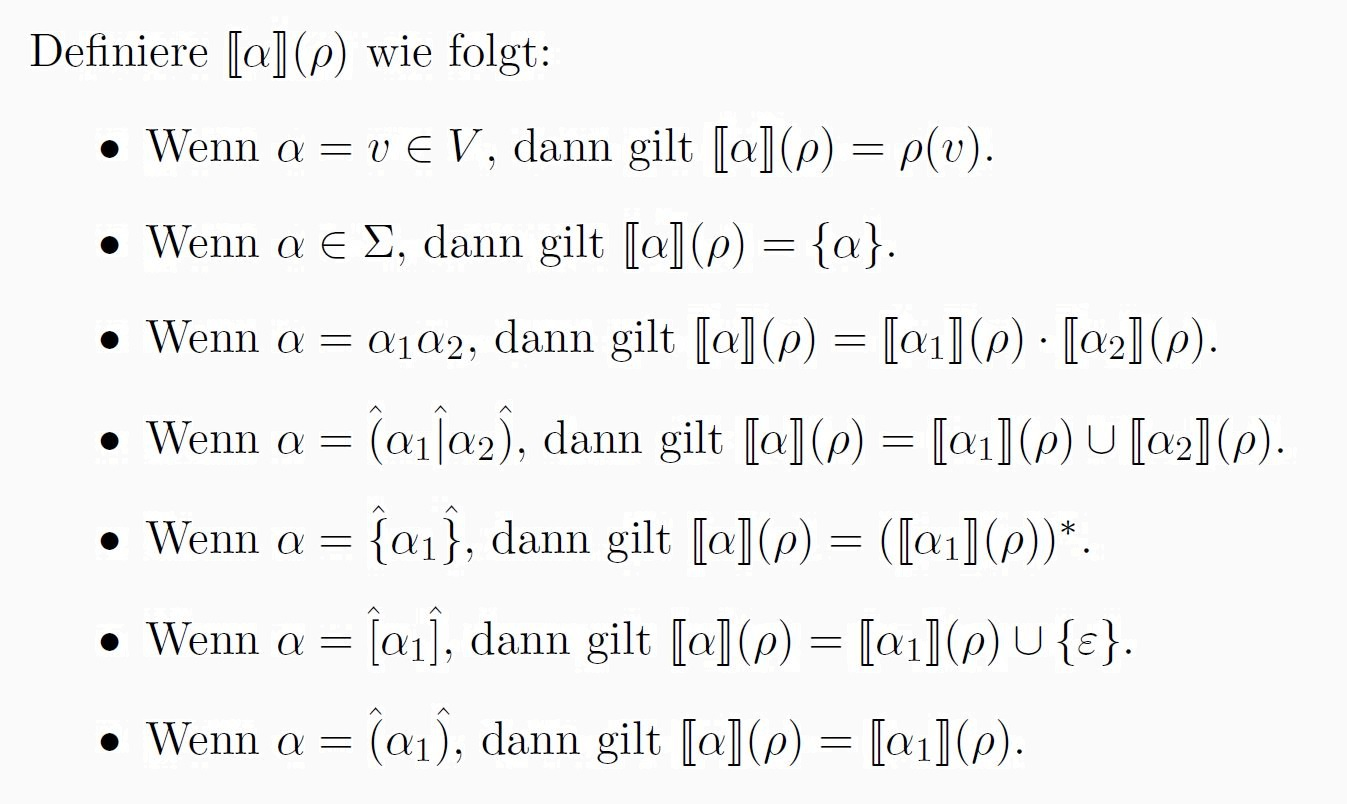
\includegraphics[width=.9\textwidth]{tut03_semantik.jpg}
	\end{itemize}	
\end{frame}

\begin{frame} \frametitle{Aufgabe 2 --- Teil (a)}
	\begin{itemize}
		\item $\rho \colon V \to \pows{\Sigma^\ast}$
		\item $f \colon (V \to \pows{\Sigma^\ast}) \to (V \to \pows{\Sigma^\ast})$
	\end{itemize}
	\pause
	\begin{align*}
		f(\rho) = \begin{pmatrix} f(\rho)(S) \\ f(\rho)(A) \end{pmatrix} 
		= \begin{pmatrix} \sem{ddAc}(\rho) \\ \sem{\byp{S}a}(\rho) \end{pmatrix} 
		&= \begin{pmatrix}
			\menge{dd} * \rho(A) * \menge{c} \\ \brackets{\rho(S) \cup \menge{\epsilon}} * \menge{a}
		\end{pmatrix} \\
		&= \begin{pmatrix}
			\menge{dd} * \rho(A) * \menge{c} \\ \rho(S) * \menge{a} \cup \menge{a}
		\end{pmatrix}
	\end{align*}
\end{frame}

\begin{frame} \frametitle{Aufgabe 2 --- Teil (b)}
	\begin{equation*}
		f(\rho) = \begin{pmatrix}
			\menge{dd} * \rho(A) * \menge{c} \\ \rho(S) * \menge{a} \cup \menge{a}
		\end{pmatrix}
	\end{equation*}
	
	\begin{align*}
		\begin{pmatrix} \emptyset \\ \emptyset \end{pmatrix}
		\mapsto^1
		\begin{pmatrix} \emptyset \\ \menge{a} \end{pmatrix}
		\mapsto^2
		\begin{pmatrix} \menge{ddac} \\ \menge{a} \end{pmatrix}
		&\mapsto^3
		\begin{pmatrix} \menge{ddac} \\ \menge{ddaca,a} \end{pmatrix} \\
		&\mapsto^4
		\begin{pmatrix} \menge{(dd)^2 (ac)^2, ddac} \\ \menge{ddaca, a} \end{pmatrix} \\
		&\mapsto^5
		\begin{pmatrix} \menge{(dd)^2 (ac)^2, ddac} \\ \menge{(dd)^2 (ac)^2 a, ddaca, a} \end{pmatrix}
	\end{align*}
\end{frame}

\begin{frame} \frametitle{Aufgabe 2 --- Teil (c)}
	Die ersten Schritte zeigten 
	\begin{equation*}
		\begin{pmatrix} \emptyset \\ \emptyset \end{pmatrix}
		\mapsto^1 \cdots \mapsto^5
		\begin{pmatrix} \menge{(dd)^2 (ac)^2, ddac} \\ \menge{(dd)^2 (ac)^2 a, ddaca, a} \end{pmatrix}
	\end{equation*}
	
	Führen wir diese Iteration nur \enquote{bis ins Unendliche} fort, so erhalten wir
	\begin{align*}
		W(\mathcal{E}, S) &= \menge{(dd)^n (ac)^n : n \ge 1} \\
		W(\mathcal{E}, A) &= \menge{(dd)^n (ac)^n a : n \ge 0}
	\end{align*}
\end{frame}


\begin{frame} \frametitle{Aufgabe 3 --- Teil (a)}
	Wir brauchen die Semantik von $S ::= \byp{a\opt{Sb}{Sbb}}$.
	\pause
		\begin{align*}
		\sem{\byp{a \opt{Sb}{Sbb}}}(\rho)
		&= \menge{\epsilon} \cup \sem{a \opt{Sb}{Sbb}}(\rho) \\
		&= \menge{\epsilon} \cup \menge{a} * \sem{\opt{Sb}{Sbb}}(\rho) \\
		&= \menge{\epsilon} \cup \menge{a} * \brackets{\sem{Sb}(\rho) \cup \sem{Sbb}(\rho)} \\
		&= \menge{\epsilon} \cup \menge{a} * \brackets{\rho(S) * \menge{b} \cup \rho(S) * \menge{bb}} \\
		&= \menge{\epsilon} \cup \menge{a} * \rho(S) * \menge{b} \cup \menge{a} * \rho(S) * \menge{bb}
	\end{align*}
	\pause
	Damit können wir die Iterationsfunktion aufstellen:
	\begin{align*}
		f(\rho) = \begin{pmatrix} f(\rho)(S) \end{pmatrix} 
		&= \begin{pmatrix} \sem{\byp{a \opt{Sb}{Sbb}}}(\rho) \end{pmatrix} \\
		&= \begin{pmatrix}
			\menge{\epsilon} \cup \menge{a} * \rho(S) * \menge{b} \cup \menge{a} * \rho(S) * \menge{bb}
		\end{pmatrix}
	\end{align*}
\end{frame}

\begin{frame} \frametitle{Aufgabe 3 --- Teil (a)}
	\begin{equation*}
		f(\rho) = \begin{pmatrix}
			\menge{\epsilon} \cup \menge{a} * \rho(S) * \menge{b} \cup \menge{a} * \rho(S) * \menge{bb}
		\end{pmatrix}
	\end{equation*}
	\pause
	
	\textbf{3 Iterationen:}
	\begin{align*}
		\begin{pmatrix} \emptyset \end{pmatrix}
		\mapsto^1
		\begin{pmatrix} \menge{\epsilon} \end{pmatrix}
		&\mapsto^2
		\begin{pmatrix} \menge{\epsilon, ab, abb} \end{pmatrix} \\
		&\mapsto^3
		\begin{pmatrix} \menge{\epsilon, ab, abb, aabb, aabbb, aabbbb} \end{pmatrix}
	\end{align*}
\end{frame}



\begin{frame} \frametitle{Aufgabe 3 --- Teil (b)}
	\small 
	Sei $\rho \colon V \to \pows{\Sigma^\ast}$ mit $\rho(S) = \menge{a^n b^n \mid 2n \ge m \ge n \ge 0}$. 
		
	\textbf{Zu zeigen:} $\sem{\byp{a \opt{Sb}{Sbb}}}(\rho) = \rho(S)$.
	
	\pause
	
	\begin{align*}
		&\sem{\byp{a \opt{Sb}{Sbb}}}(\rho) \\
		= \enskip & \menge{\epsilon} \cup \menge{a} * \rho(S) * \menge{b} \cup \menge{a} * \rho(S) * \menge{bb} \\
		= \enskip & \scalebox{0.8}{ $\menge{\epsilon} \cup \menge{a} * \menge{a^n b^n \mid 2n \ge m \ge n \ge 0} * \menge{b} \cup \menge{a} * \menge{a^n b^n \mid 2n \ge m \ge n \ge 0} * \menge{bb} $} \\
		= \enskip & \menge{\epsilon} \cup \menge{a a^n b^n b \mid 2n \ge m \ge n \ge 0} \cup \menge{a a^n b^m bb \mid 2n \ge m \ge n \ge 0}  \\
		= \enskip & \menge{a^n b^m \mid 2n \ge m \ge n \ge 0} \\
		= \enskip & \rho(S)
	\end{align*}
\end{frame}



\end{document}